
\section{Introduction}


\begin{frame}
\frametitle{Initial Overview}

\begin{itemize}[<+->]
  \item The B method supports the construction of safety systems
  \begin{itemize}
    \item From design model
    \item To implementation model
    \item But part of this translation is not guaranteed by formal means\\
    \begin{center}
       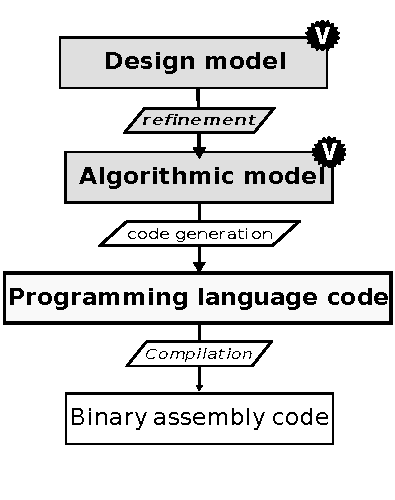
\includegraphics[height=.5\textheight]{figures/b-method-actual_new.pdf}
    \end{center}
       \begin{itemize} \item   \small{The transformation process can introduce small bugs}
       \end{itemize}
  \end{itemize}
\end{itemize}
   

	\note{ ................... }
	
\end{frame}



\begin{frame}
\frametitle{Extended Overview}  

\begin{itemize}%[<+->]
    \item We proposed a approach [Dantas, 2008] to extend the formal
    verification
    \item One key element of this approach is the formal model of the
    instruction set of execution platform % of such assembly languages
     \\ \begin{center}     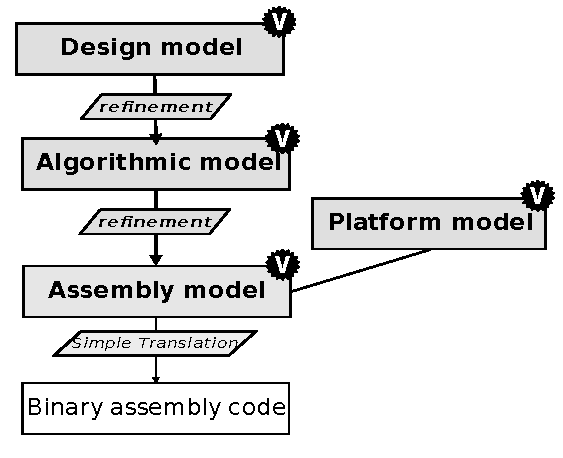
\includegraphics[height=.5\textheight]{figures/b-method-ideal_new.pdf} \end{center}
\end{itemize}
	\note{...................}
\end{frame}


\begin{frame}
\frametitle{Modelling Assembly Instruction Set in B}  

\begin{itemize}[<+->]
  \item We developed libraries with definitions of hardware and integer types
	%.The modelling is builded using some  developed libraries
  \item The libraries have common concepts that can be used to others platforms of 8 or 16 bits
  \item Utilities of this formal model:
  \begin{itemize}
    \item Documentation
    \item Simulation
    \item Reference for verification of Z80 hardware implementations 
    \item The formal verification to the assembly level
    %\item A possible support to verify the Z80 design


  \end{itemize}
\end{itemize}

	\note{ ................... }
\end{frame}


% 
% \begin{frame}
% \frametitle{Objective}  
% 
% \begin{itemize}[<+->]
%   \item The main actual objective is represent the assembly instruction set
%     \begin{itemize}
%     \item The aspects no-functional are not represented: logic circuits, pipeline, data bus, \ldots 
%   \end{itemize}
%   \item Moreover there are many efficient ways to verify hardware
% 
% \end{itemize}
% % 
% 
% 	\note{ ................... }
% \end{frame}
% 


